\chapter{Results \& Discussion}

\textbf{Should include a reiteration of the experiments, and their outcome.  Together with a description (discussion).  Preamble should include a reminder of the aims and objectives together with a list of experiments to achieve these.  Should include many charts and other visualization with appropriate descriptions}.  


% Paper on biological replicates https://www.ncbi.nlm.nih.gov/pmc/articles/PMC4878611/
% An RNA-seq experiment with 48 biological replicates in each of two conditions was performed to answer these questions and provide guidelines for experimental design. With three biological replicates, nine of the 11 tools evaluated found only 20%–40% of the significantly differentially expressed (SDE) genes identified with the full set of 42 clean replicates

%Discuss the FDR error rate. 5% of our DEGs are false positives

\section{Determining the Optimal Tools}

The following is the reasoning behind the final decisions made on the tool choices of each step of the pipeline, based on the literature reviewed. Extensive descriptions of the final tools implemented in the pipeline can be found throughout Section \ref{RNA-seq: in silico}.
% NOTE SEE IF U NEED TO CHANGE THIS. Maybe group all the tools in a single place

Tools which measure quality metrics without altering the data require little justification for their use, their mention occasionally being completely omitted from RNA-seq studies \autoref{tab:rnaseq_experiments}. \textbf{FastQC} is a staple of sequencing quality control, providing a detailed analysis of the contents of FASTQ files and drawing attention to signs of low quality reads. While FastQC results are detailed, they lack the detection of external nucleotide contaminants in the data. This information was supplemented with the results from \textbf{FastQScreen} which aligns the experimental sequences to common contaminant sequences (e.g. mouse, \textit{Drosophila}, rRNA) and provides a graph marking any successful alignments.

To trim the data, we have chosen \textbf{Cutadapt}, which pipes its output back to FastQC through the wrapper script \textbf{Trim Galore!}. Additional filtering was performed by \textbf{Prinseq++} which may detect and remove regions of low-complexity. The functionality of these tools were found to complement each other. Filtering and trimming the data at this stage was relatively unimportant, as suggested by the findings of \cite{he2020assessing} and because the raw data of this project was of good quality to begin with. \cite{liao2020read} doubt the necessity of trimming at all.

Despite \textbf{STAR} needing a lot of RAM \citep{Dobin2013} and being slower than more light-weight aligners \citep{srivastava2020alignment}, these were not limiting factors due to our access to a High Performance Computer (HPC) and small number of samples. \cite{srivastava2020alignment} found that the choice between quasi-mappers (e.g. Salmon) and traditional aligners (e.g. STAR) is a trade-off between speed and accuracy. Similarly \cite{Zhang2017} found that pseudo-aligners Salmon and Kallisto require less runtime while maintaining similar accuracy to STAR. \cite{Schaarschmidt2020} find that the effect aligners have on the final list of \ac{DEG}s is negligible, and that all tested aligners can be used equally for RNA-seq. Even if STAR provides a marginal increase in accuracy over quasi-aligners, this is preferred over the improvements in speed or computational resources provided by other aligners.

The most difficult and time-consuming choice to make was the tool to perform differential gene expression. The invested effort was justified by the findings of \cite{williams2017empirical}, which state that the method of \ac{DGE} exhibits the strongest impact on the results. Our data consists of three time points (1hr, 6hr, 12hr) and a control, each lacking replicates. Since we cannot accurately estimate the variance or dispersion with a single reading, many \ac{DGE} tools simply fail to function. Although one may argue that this is not a major issue due to the negligible technical variance of RNA-seq \citep{bullard2010evaluation} and the minimal biological variance in our data which is derived from the same \ac{ATRA}-resistant HL-60 cell line.

Due to the lack of review papers and benchmarks comparing the tools which claim to function well without replicates, they were manually tested and investigated (see Section \ref{DGE no replicates}). The lesser-known tools (GFOLD, LPESeq, DEGseq, IsoDE), while developed specifically to function without replicates, were found to be limited in functionality when compared to \textbf{edgeR}. Additionally, due to their rather unconventional approach to \ac{DGE}, their output was found to be incompatible with other downstream libraries, limiting the potential for data exploration. The decision between 

EdgeR has multiple methods to determine which genes are differentially expressed (\autoref{edger_dge_options}). The likelihood ratio tests \citep{mccarthy2012differential} compared values against their mean, which was not applicable to our study because we needed to compare reads from treated cells against reads from untreated cells. Quasi-likelihood F-tests \citep{lun2016s, lund2012detecting} were simply not applicable to datasets lacking replicates, which leaves us with the classic exact test for the negative binomial distribution \citep{robinson2007moderated, robinson2008small}. This is a pairwise test which compares the means between two groups of counts, applicable to experiments with a single factor. It hould not be confused

\citep{robinson2007moderated, robinson2008small}, or the Generalized Linear Model (GLM) route, although certain features of the two may be combined. The GLM tests for \ac{DGE} are likelihood ratio tests (LRTs)  and quasi-likelihood F-tests (QLFs) \citep{lun2016s, lund2012detecting}.

The GLM tests for DGE are likelihood ratio tests (LRTs) (McCarthy et al.,
2012) and quasi-likelihood F-tests (QLFs) 

 but the classic \texttt{exactTest} was deemed as most appropriate. 

 Two primary routes may be taken using \autoref{fig:edger_options}, the classic route which involves exact tests \citep{robinson2007moderated, robinson2008small}, or the Generalized Linear Model (GLM) route, although certain features of the two may be combined. The GLM tests for \ac{DGE} are likelihood ratio tests (LRTs) \citep{mccarthy2012differential} and quasi-likelihood F-tests (QLFs) \citep{lun2016s, lund2012detecting}.

The \texttt{exactTest} function is based on quantile-adjusted conditional maximum likelihood (qCML) method. It produces a matrix of pseudo-counts\footnote{Note that the meaning of the term \textit{pseudo-counts} may change according to the context, and may be used by other studies to refer to something different.} which are designed to speed up computational analysis and not to be interpreted as regular normalised counts. The qCML method is only applicable on datasets with a single factor.


\subsubsection{Adapting DGE Analysis to a Lack of Replicates}
\label{DGE no replicates}

The accuracy of any statistical analysis is dependent on the number of replicates. Technical replicates allow the isolation of the non-biological variation to evaluate the quality of the instruments and methodology used. Biological replicates originate from different biological sources and are meant to test the biological variance of the samples. \cite{liu2014rna} find that in RNAseq biological variation is by far more important, and given a choice between the two, the researcher should invest in biological replicates. \cite{bullard2010evaluation} confirm this claim, finding that technical variation in RNAseq experiments is minimal. \cite{schurch2016many} found that using three biological replicates gave 20\% to 40\% of the \ac{DEG}s (varies according to the tool) compared to a full set of 42 replicates (representing the 'true' population). This rises to >85\% when considering genes with a log$_2$ fold change of >2. \cite{schurch2016many} state that ideally an RNAseq experiment for \ac{DGE} should have a minimum of six replicates per condition for all experiments and 12 replicates for experiments where the identification of \textit{all} the \ac{DEG}s, even the lowly expressed ones, is important. 

However, in practice, performing an experiment with large numbers of replicates is not always possible. Budget constraints and the still-high cost of sequencing are a common issue in RNAseq experiments. To make the most of such datasets, several \ac{DGE} tools advertise their ability to work with just a single reading per experimental condition \citep{feng2012gfold, gim2016lpeseq, anders2010differential, wang2010degseq, al2014bootstrap}. Notably, DESeq2 does not support datasets without replicates. There is an unfortunate lack of review papers and independent studies which benchmark these tools, except for brief comments in \cite{schurch2016many} who recommend edgeR (\texttt{exactTest}) or DESeq2 for experiments with <12 replicates per condition. For this reason this section will be reviewing the available tools adapted to performing \ac{DGE} without replicates.

The first tool in this review will be \textbf{GFOLD} \citep{feng2012gfold}, developed specifically for datasets lacking in replicates. The developers acknowledge the dependence of \textit{p}-values on variance estimation, which is impossible without replicates. A unique GFOLD value replaces the standard metrics of significance (\textit{p}-values) and expression change (log$_2$ fold changes). \cite{feng2012gfold} describe the value as a relative change of the expression level. GFOLD is unique in that it is the only tool in this comparison that is called through the Linux command line, instead of being an R library.

\textbf{LPESeq} \citep{gim2016lpeseq} introduces the Local-Pooled-Error (LPE) method for few or single-replicate \ac{DGE} analysis. This method attempts to estimate transcript-specific variance using the raw values of each transcript per condition. Hypothesis testing for significant difference is then performed to identify the differentially expressed genes.

\textbf{IsoDE} \citep{al2014bootstrap} is a non-parametric method (i.e. it assumes no statistical distribution) and is based on bootstrapping. The algorithm generates FPKM estimates from read counts of each condition which undergo pairwise comparison.

An MA-plot-based method, the R library \textbf{DEGseq} \citep{wang2010degseq} (not to be confused with DESeq) accepts input .bed or .eland input files and outputs an XHTML page with \textit{p}-values, gene expression values and expression differences in the form of Q-values.

The final tool in this review is the Bioconductor R library \textbf{edgeR} \citep{edger}. It may be more accurately described as a collection of methods, neither of which are specifically adapted to data without replicates, but the documentation provides recommendations to adapt the analysis to with the lack of replicates. EdgeR and its normalisation technique TMM have already been covered extensively in Section \ref{EdgeR} and Section \ref{TMM} respectively. 
% Describe edger no replicates here

% really perfect paper https://www.ncbi.nlm.nih.gov/pmc/articles/PMC4878611/#:~:text=Recommendations%20for%20RNA%2Dseq%20experiment%20design&text=At%20least%20six%20replicates%20per,all%20DE%20genes%20is%20important.





\section{Assessing the Quality of the Raw Data}
\label{Assessing the Quality of the Raw Data}
We started off with four single-ended 50bp FASTQ files, one per experimental time point (control, 1hr, 6hr, 12hr). Paired-end reads of longer length (perhaps 150bp) would have been more accurate, although on their website, Illumina suggests that these are more affordable and sufficient for a \ac{DGE} RNA-seq experiment \citep{illumina2022reads}.



\subsection{FastQC}
Figure \ref{fig:fastqc-status-check-heatmap} shows the FastQC results for each raw file, summarised as a heatmap generated by MultiQC. Caution should be exercised when interpreting RNA data through FastQC, as the program is primarily calibrated to DNA data. Two modules failed consistently throughout the four samples received: \textit{Sequence Duplication Levels} and \textit{Per base sequence content}.
This is normal and expected even for high-quality RNA, as explained in a tutorial by Michigan State University \citep{fastqctutorial2021}.

An inherent quality of RNA data which makes \ac{DGE} possible, is that transcripts are unevenly distributed across genes. These highly abundant reads are detected as duplicate sequences. As a benign artefact of library preparation, the first 10-15 bases of RNA reads are expected to be non-uniformly distributed, causing the module to fail \citep{fastqctutorial2021}.

%copy paste the definitions for the modules from lit review lol

\begin{figure}[!h]
    \centering
    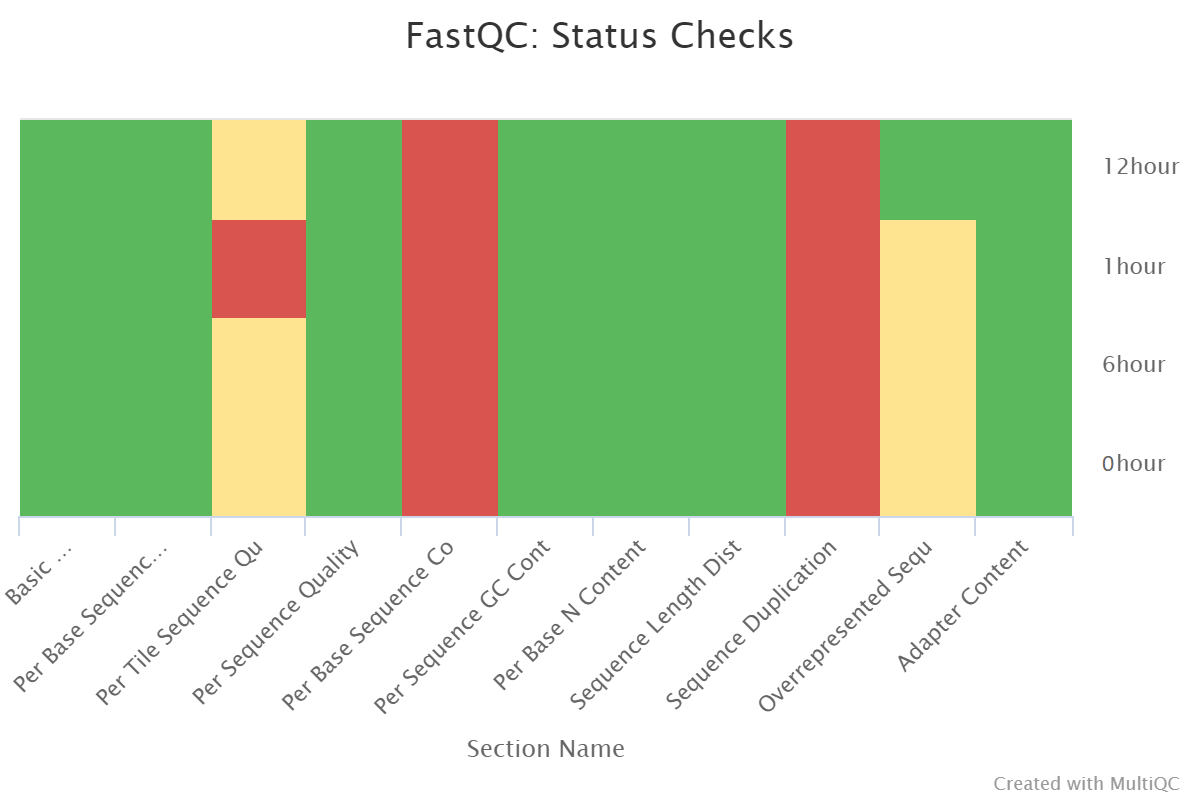
\includegraphics[width=1\textwidth]{fastqc-status-check-heatmap}
    \caption[Heat map showing the status of each FastQC module]{Heat map generated by MultiQC showing the status of each FastQC module: Pass, Warning or Fail.} 
    \label{fig:fastqc-status-check-heatmap}
\end{figure}

\begin{figure}[!h]
    \centering
    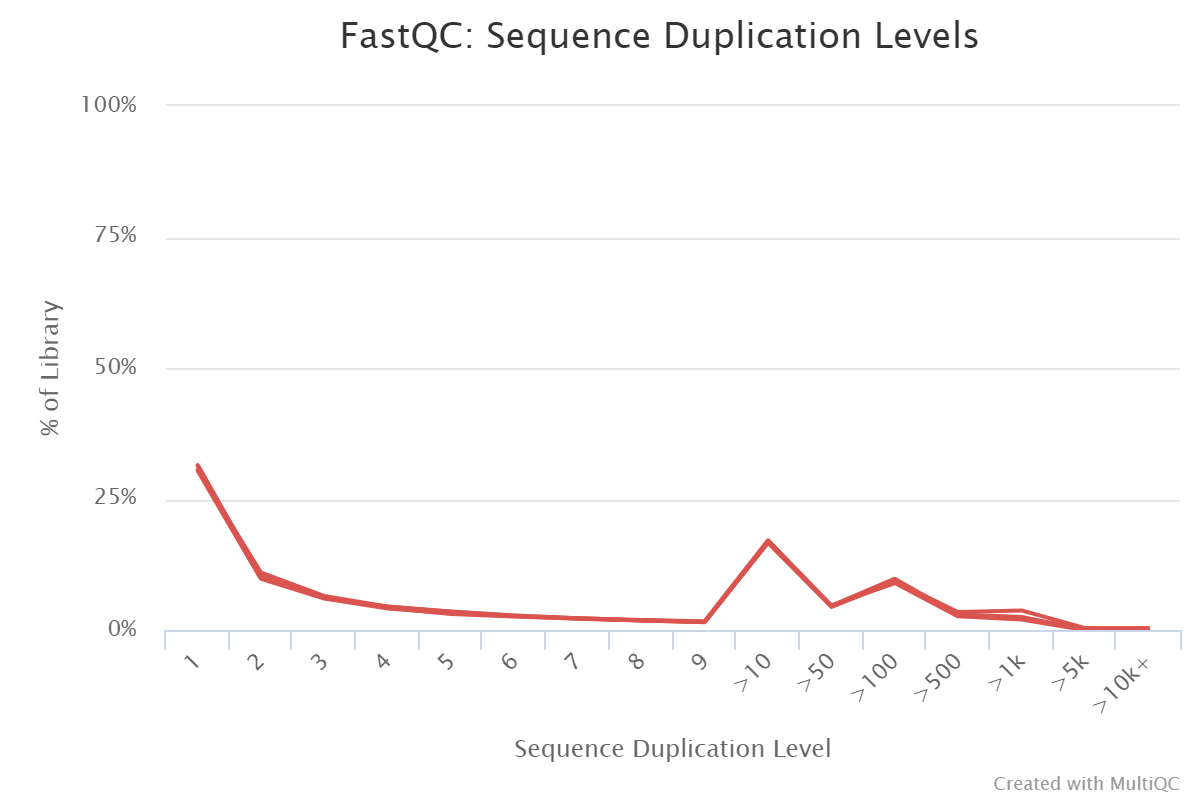
\includegraphics[width=1\textwidth]{fastqc_sequence_duplication_levels_plot}
    \caption[Sequence duplication levels plots for all samples]{Sequence duplication levels plots for all samples, showing the wide range of possible coverages in RNA data, ranging from 1 to >10,000.} 
    \label{fig:fastqc_sequence_duplication_levels_plot}
\end{figure}


\begin{figure}[!h]
    \centering
    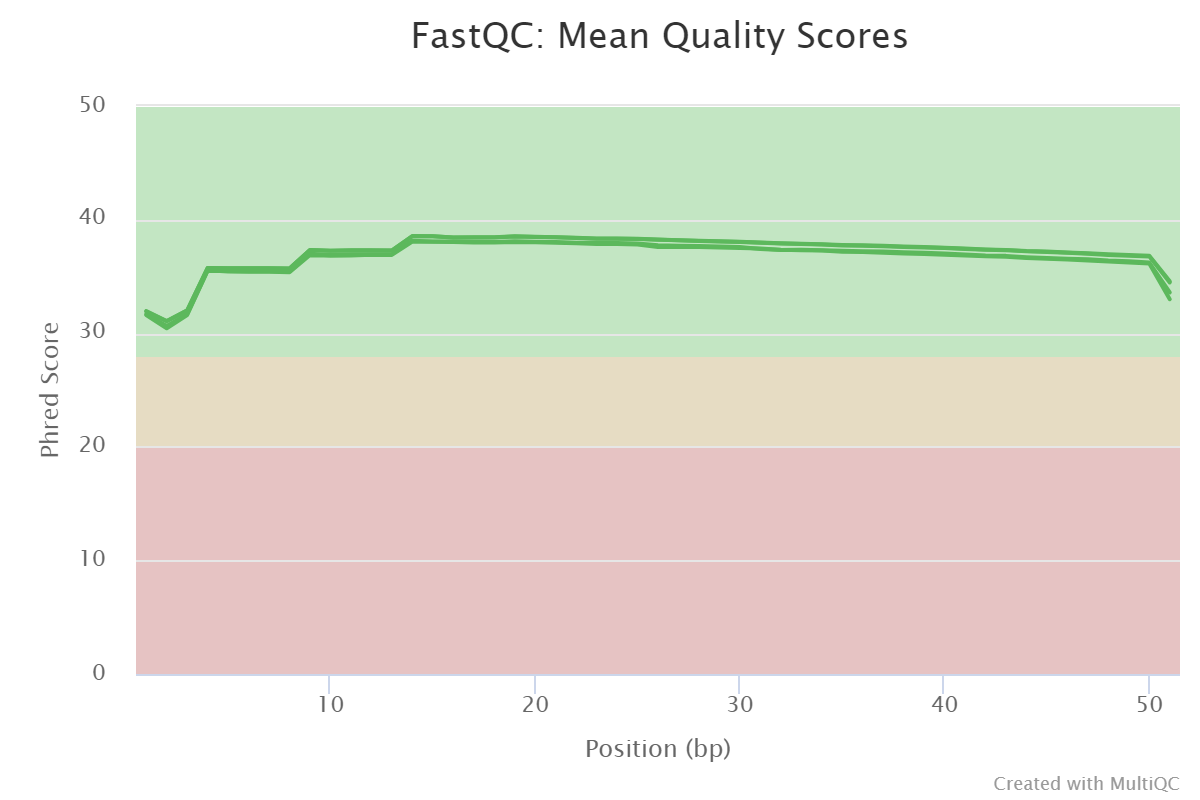
\includegraphics[width=1\textwidth]{fastqc_per_base_sequence_quality_plot}
    \caption[]{}
    \label{fig:fastqc_per_base_sequence_quality_plot}
\end{figure}

\begin{figure}[!h]
    \centering
    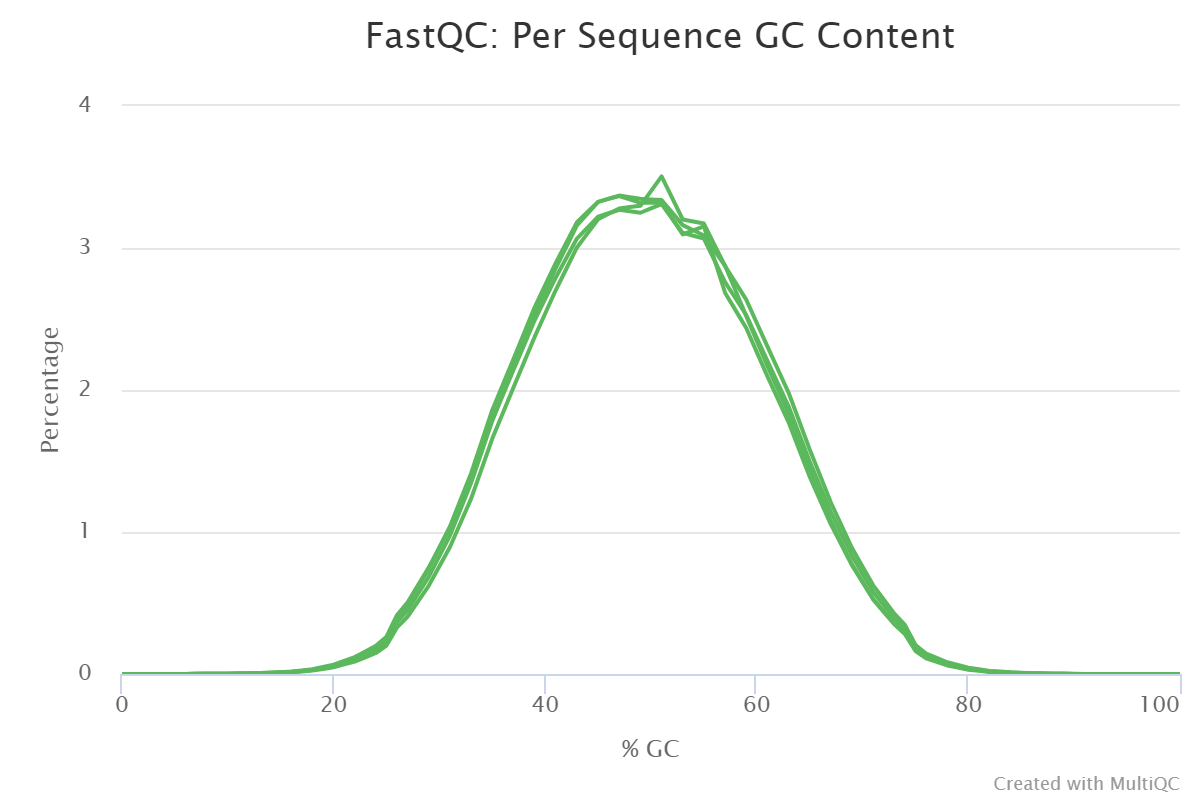
\includegraphics[width=1\textwidth]{fastqc_per_sequence_gc_content_plot}
    \caption[]{}
    \label{fig:fastqc_per_sequence_gc_content_plot}
\end{figure}

\begin{figure}[!h]
    \centering
    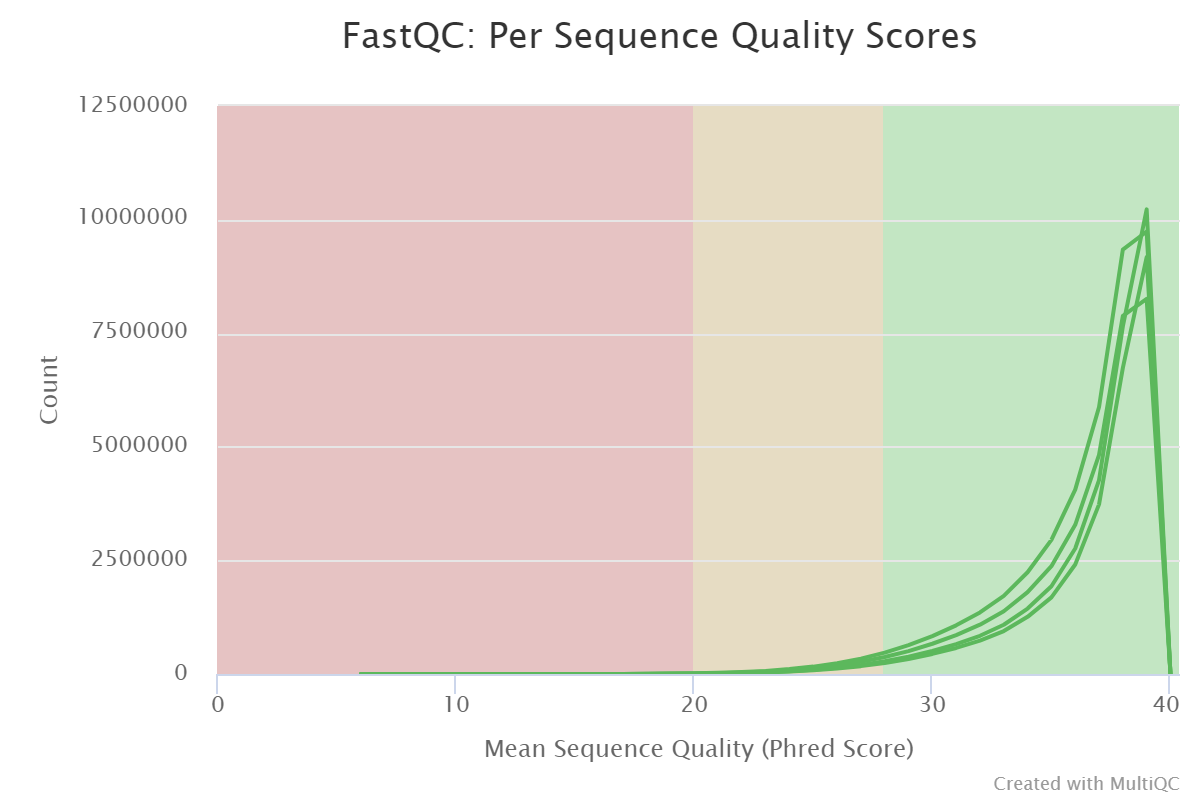
\includegraphics[width=1\textwidth]{fastqc_per_sequence_quality_scores_plot}
    \caption[]{}
    \label{fig:fastqc_per_sequence_quality_scores_plot}
\end{figure}

\begin{figure}[!h]
    \centering
    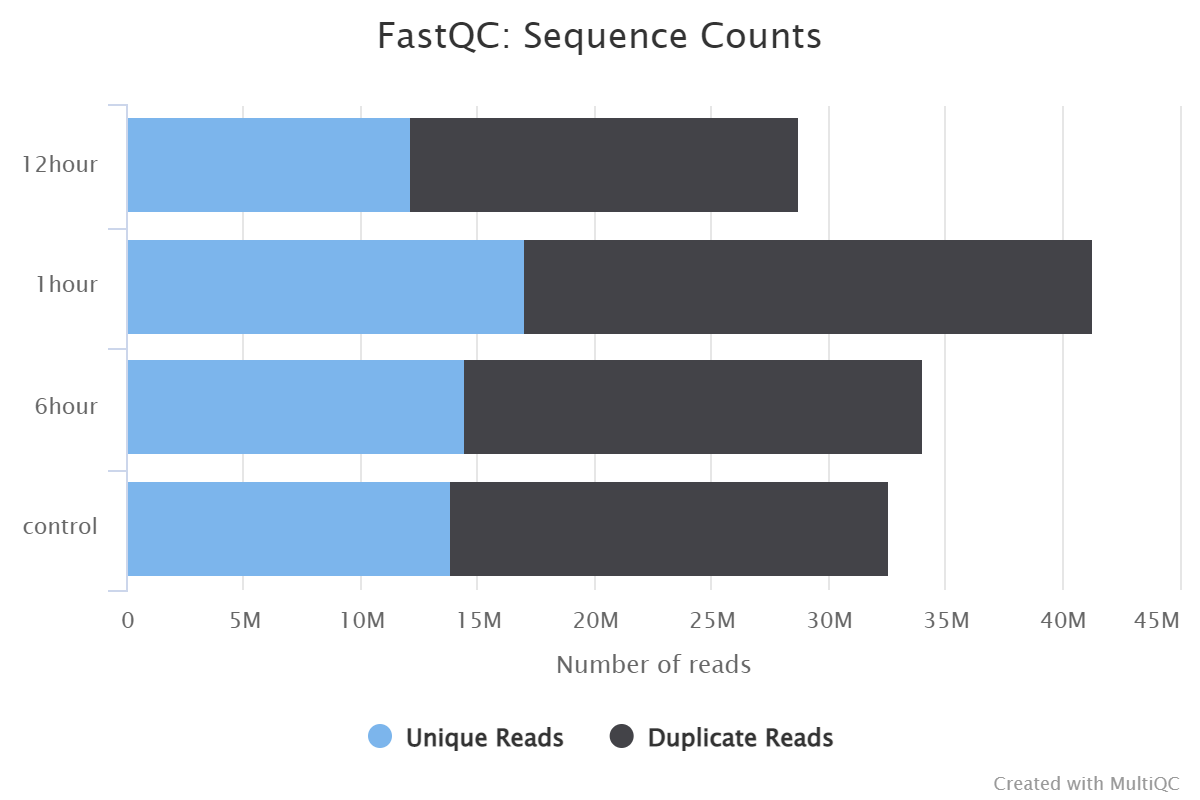
\includegraphics[width=1\textwidth]{fastqc_sequence_counts_plot}
    \caption[]{}
    \label{fig:fastqc_sequence_counts_plot}
\end{figure}

\begin{figure}[!h]
    \centering
    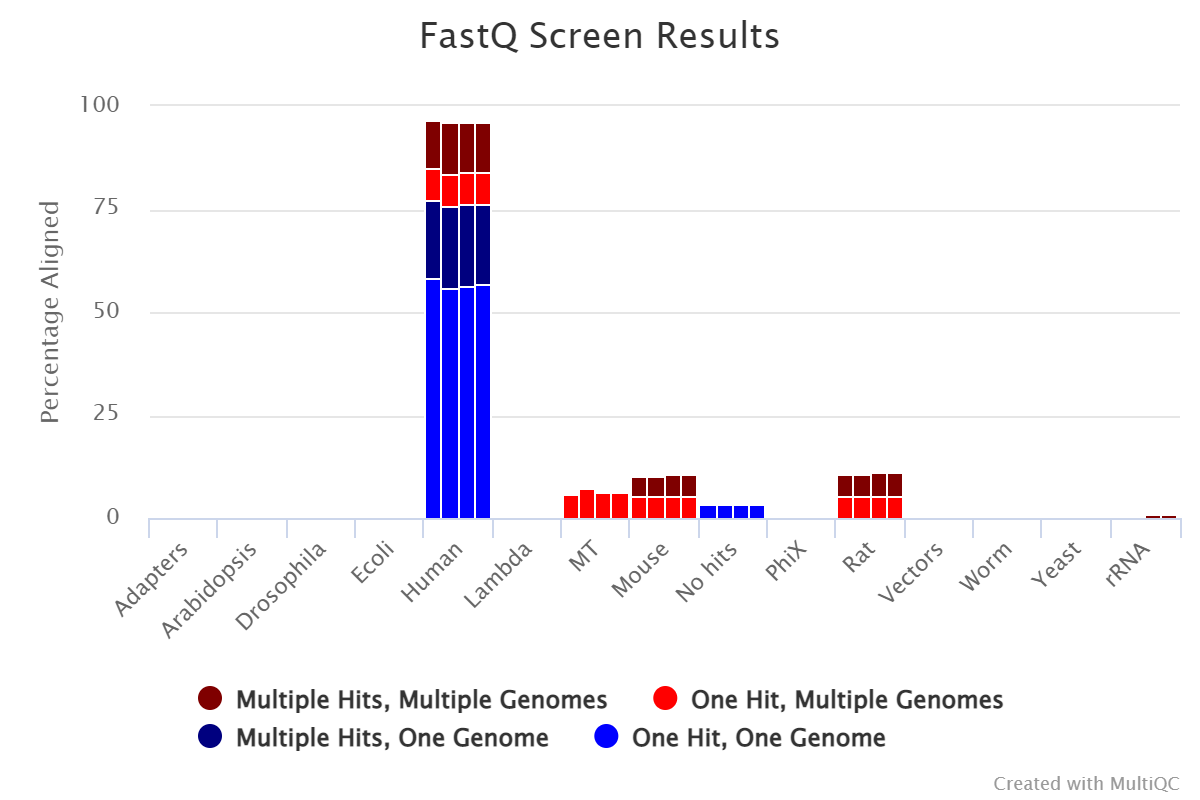
\includegraphics[width=1\textwidth]{fq_screen_plot}
    \caption[FastQ Screen plot showing what percentage of the reads aligned to which genome(s)]{FastQ Screen plot showing what percentage of the reads aligned to which genome(s). The samples show signs of good quality. There is an almost 100\% successful alignment to the human genome, with some alignment to other sequences which share common sequences. Some degree of multi-mapping (20\%) with the human reference is present.} 
    \label{fig:fq_screen_plot}
\end{figure}




\section{Preprocessing}
FastQC detected traces (<0.5\%) of TruSeq adapters in the FASTQ files, which is corroborated by the sequencer's manual \citep{HiSeq2000} stating that it makes use of the 'TruSeq family of reagents'. Adapter sequences were trimmed, and resultant reads which were <45 bp long were removed. Between 1.3 and 1.6\% of the base-pairs were trimmed across the four samples.


\begin{figure}[!h]
    \centering
    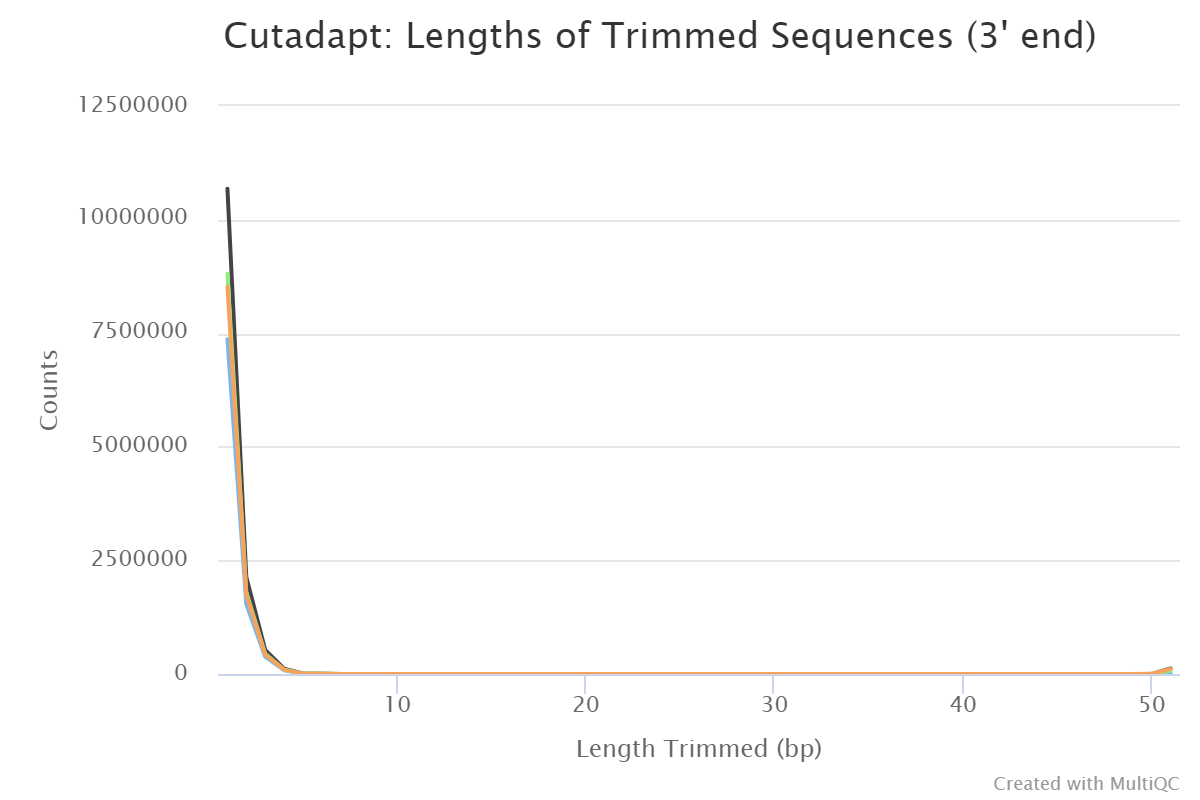
\includegraphics[width=1\textwidth]{cutadapt_trimmed_sequences_plot_3}
    \caption[Heat map showing the status of each FastQC module]{Heat map showing the status of each FastQC module: Pass, Warning or Fail.} 
    \label{fig:cutadapt_trimmed_sequences_plot_3}
\end{figure}

Prinseq++ (check log files)

\section{Alignment}

\begin{figure}[!h]
    \centering
    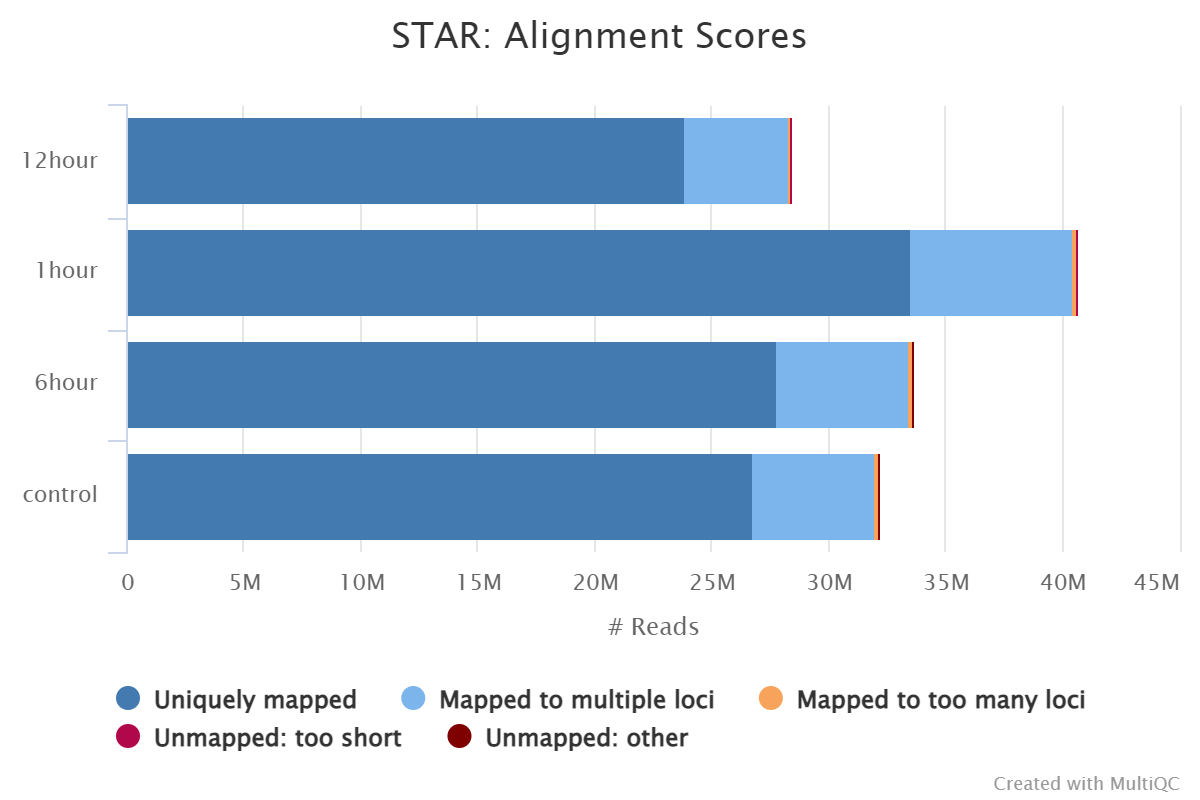
\includegraphics[width=1\textwidth]{star_alignment_plot}
    \caption[Heat map showing the status of each FastQC module]{Heat map showing the status of each FastQC module: Pass, Warning or Fail.} 
    \label{fig:star_alignment_plot}
\end{figure}




\section{QC Summary}
\begin{table}[!ht]
    \centering
    \begin{tabular}{|l|l|l|l|l|l|l|}
    \hline
        Sample Name & \% Aligned & BP Aligned (M) & \% BP Trimmed & \% Duplicates & \% GC & Total seqs (M) \\ \hline
        12hour & 83.8\% & 23.9 & 1.3\% & 57.7\% & 49\% & 28.8  \\ \hline
        1hour & 82.2\% & 33.5 & 1.6\% & 58.9\% & 48\% & 41.3  \\ \hline
        6hour & 82.6\% & 27.8 & 1.5\% & 57.5\% & 49\% & 34.1  \\ \hline
        control & 83.1\% & 26.8 & 1.6\% & 57.6\% & 49\% & 32.6  \\ \hline
     \end{tabular}
\end{table}



% https://hbctraining.github.io/Intro-to-rnaseq-hpc-salmon/lessons/qc_fastqc_assessment.html
% Really good resource on RNAseq QC
% The next plot gives the “Per base sequence content”, which always gives a FAIL for RNA-seq data. This is because the first 10-12 bases result from the ‘random’ hexamer priming that occurs during RNA-seq library preparation. This priming is not as random as we might hope giving an enrichment in particular bases for these intial nucleotides.
% The “Per sequence GC content” plot gives the GC distribution over all sequences. Generally is a good idea to note whether the GC content of the central peak corresponds to the expected % GC for the organism. Also, the distribution should be normal unless over-represented sequences (sharp peaks on a normal distribution) or contamination with another organism (broad peak). This plot would indicate some type of over-represented sequence with the sharp peaks, indicating either contamination or a highly over-expressed gene.
% The next module explores numbers of duplicated sequences in the library. This plot can help identify a low complexity library, which could result from too many cycles of PCR amplification or too little starting material. For RNA-seq we don’t normally do anything to address this in the analysis, but if this were a pilot experiment, we might adjust the number of PCR cycles, amount of input, or amount of sequencing for future libraries. In this analysis we seem to have a large number of duplicated sequences, but this is expected due to the subset of data we are working with containing the over-expression of MOV10.
%

 %Another one: https://rtsf.natsci.msu.edu/genomics/tech-notes/fastqc-tutorial-and-faq/#:~:text=FastQC%2C%20written%20by%20Simon%20Andrews,on%20a%20sequence%20data%20set.


% INTERNPRETING FASTQC REPORT NOTES:
% Real good resource of possible explanations:
% We have positional sequence bias: https://sequencing.qcfail.com/articles/positional-sequence-bias-in-random-primed-libraries/
% High Sequence Duplication levels are expected: https://www.biostars.org/p/307361/
%From Molecular Biology assignment:
%  One cycle per base pair would have been needed, so 50 cycles should have been performed.
%
% The sample has a 48 %GC, which is within the expected range for a human genome. 
% As a result of an additional hydrogen bond and especially because of increased base 
% stacking effects, GC base pairs experience stronger bonding. Consequently, during PCR, 
% endonucleases are less likely to cleave these bonding pairs, hindering the quality if the 
%GC is high. GC bias occurs in both GC-rich and GC-poor fragments as the effect of 
% GC content is unimodal.
%
%The quality of the base calls peaks around the 14th and 15th base pair, then gradually 
%declines. This is a result of phasing, a type of sequencing error which causes reads to 
%become out-of-sync. This can occur by two similar phenomena: pre-phasing and postphasing. Pre-phasing occurs when two or more nucleotides bind to the read in a single 
%cycle, causing the sequence to ‘skip’ a nucleotide. This often occurs when the flow-cell is 
%not flushed properly or in the case of a defect terminator cap. Post-phasing is caused by 
%the incomplete removal of the terminator cap, leading to the sequence lagging behind 
%the rest of the cluster. As more cycles go by, the higher the probability of an error to 
%occur which causes the read to become out of phase, and when this occurs, it will pollute 
%the light signals of all subsequent cycles.


\begin{table}[]
\centering
\caption{How read counts change through the pipeline filtering steps}
\label{tab:read_counts}
\begin{tabular}{cclll}
\hline
                                                                   & \textbf{Control} & \textbf{1 hour} & \textbf{6 hour} & \textbf{12 hour} \\ \hline
Unfiltered                                                         & 32.62M           & 41.30M          & 34.08M          & 28.77M           \\ \hline
\begin{tabular}[c]{@{}c@{}}Trimming \\ (Trim Galore!)\end{tabular} & 32.23M           & 40.81M          & 33.71M          & 28.54M           \\ \hline
\begin{tabular}[c]{@{}c@{}}Filtering\\ (Prinseq++)\end{tabular}    & 32.22M           & 40.75M          & 33.66M          & 28.50M           \\ \hline
\begin{tabular}[c]{@{}c@{}}Alignment \\ (STAR)\end{tabular}        & 26.80M           & 33.54M          & 27.78M          & 23.89M           \\ \hline
\end{tabular}
\end{table}



\subsection{Preprocessing}


%Explain that RSEM had the option to perform the alignment via another aligner (eg STAR), but sacrificed flexibility so it was decided that keeping the alignment and quantification as seperate steps was better



% Sorting BAM by read name vs by coordinate (I chose coordinate)
% 

\subsection{Determining the Normalisation method}
%TMM vs TPM vs both
% Both were attempted: TMM resulted in a total of x DEG while TPM resulted in 100 DEG.
% The edgeR vignette suggests to use the raw counts (?) of RSEM for normalisation, as opposed to using the already normalised TPM so we went with this.
 % FPKM/RPKM are not good measures of relative abundance because the FPKM/RPKM of a transcript can change between two samples even if its relative abundance stays the same.
% https://groups.google.com/g/rsem-users/c/GRyJfEOK1BQ <- very good explanation 

\subsection{Accounting for Multiple testing}
%FDR
%Benjamini Hochback 

\section{Pathway analysis}

\subsection{Biological Interpretation of Pathways showing Differential Expression}

% https://www.biostars.org/p/9510180/ reply says that even though a gene is downregulated, it might be suppressing other genes in the pathway which makes the other genes indirectly upregulated. Keep stuff like this in mind when interpreting gene expression.


\section{Interpretation of Results}


% 1 hour was an outlier. Hypothesis: Cells which were differentiated died off (degrading their RNA) while others proliferated
% this is supported by the literature. Check if apoptosis pathways for the 6hr and 12hr are activated as opposed to differentiation pathways of the 1hr
% We dont know how long this differentiation > apoptosis thing takes. The 1hr might be in the middle of apoptosis and/or differentiation. 6hr and 12hr the cells might have stabilised. Check pathways to be sure. 

% Problems with the reference genome: https://genomebiology.biomedcentral.com/articles/10.1186/s13059-019-1774-4

\section{Summary}
\enlargethispage{\baselineskip} % so you do not get a single line in another page